\chapter{RESEARCH METHODOLOGY}
\label{chap:3}

\section{Research Framework}
\label{sec:research-framework}

This research proposes a deep learning-based framework for automated analysis of CMR images to support myocardial infarction assessment. The network integrates cardiac structure segmentation, myocardial scar assessment, and quantitative scar area measurement into a unified workflow. Instead of treating these tasks as independent processes, the output generated at each stage serves as the input for the subsequent stage, establishing a systematic framework for myocardial infarction assessment. The overall research method is presented in Figure~\ref{fig:ch3-research-stages} \citep{Ronneberger2015,Bernard2018,Zhuang2020}.

The proposed framework utilizes two publicly available CMR datasets with different roles. The Automated Cardiac Diagnosis Challenge (ACDC) dataset is used for cardiac structure segmentation because it provides expert annotations of the left ventricle, right ventricle, and myocardium at both End-Diastole (ED) and End-Systole (ES). Subsequently, the Myocardial Pathology Segmentation (MyoPS2020) dataset is used for myocardial scar assessment based on complementary multi-sequence CMR images, including balanced steady-state free precession (bSSFP), T2-weighted imaging (T2WI), and Late Gadolinium Enhancement (LGE). The use of these two datasets enables each stage of the proposed framework to be developed using data that are specifically designed for its corresponding objective \citep{Bernard2018,Zhuang2020}.

The framework begins with cardiac structure segmentation using a U-Net-based architecture to identify the left ventricle, right ventricle, and myocardium from cine CMR images. To establish a reliable segmentation framework, the proposed method investigates the activation function, pooling strategy, and loss function while maintaining a consistent network architecture throughout the experiments. The resulting myocardium segmentation subsequently defines the anatomical region used for myocardial scar assessment, thereby establishing the anatomical foundation for the subsequent scar analysis \citep{Ronneberger2015,Diamantis2020,Riandini2025Array}.

Following cardiac structure segmentation, myocardial scar assessment is performed using the MyoPS2020 dataset. Rather than transferring segmentation masks between datasets, the anatomical knowledge established through the cardiac structure segmentation framework is independently applied to define the myocardium region for myocardial scar assessment within the MyoPS2020 dataset, thereby providing the anatomical region used for subsequent myocardial scar analysis.

Finally, the proposed framework is evaluated using quantitative performance metrics appropriate for both segmentation and scar area quantification. The methodology presented in this chapter provides the foundation for the implementation and experimental investigations described in Chapters IV, V, and VI.

\begin{figure}[htbp]
	\centering
	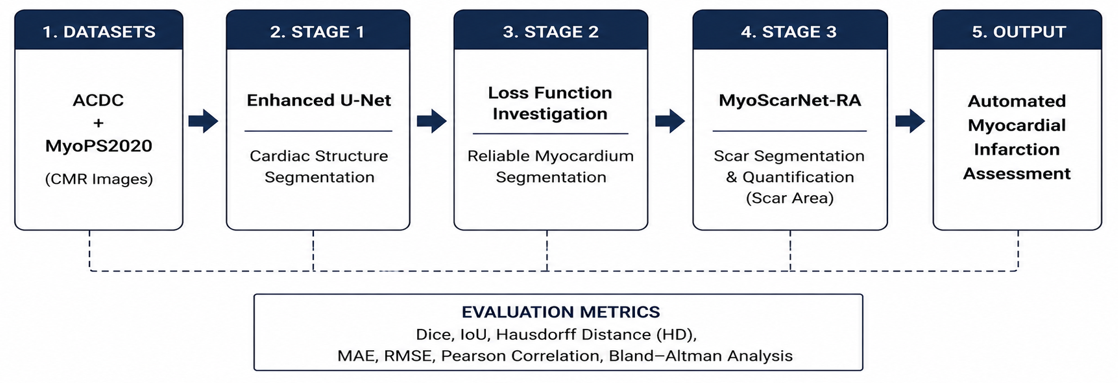
\includegraphics[width=0.86\textwidth]{bab3/ch3-research-stages.png}
	\caption{Overall Research Framework of the Proposed Deep Learning-Based CMR Image Analysis for Myocardial Infarction Assessment}
	\label{fig:ch3-research-stages}
\end{figure}

\section{Research Dataset and Dataset Preparation}
\label{sec:dataset-preparation}

This research utilizes two publicly available CMR datasets, namely the Automated Cardiac Diagnosis Challenge (ACDC) dataset and the Myocardial Pathology Segmentation (MyoPS2020) dataset. Before model development, each dataset was prepared according to the requirements of its respective study. The ACDC dataset was prepared for cardiac structure segmentation in Chapters IV and V, whereas the MyoPS2020 dataset underwent an independent preparation procedure for myocardial scar segmentation and quantitative scar assessment in Chapter VI.

\subsection{Automated Cardiac Diagnosis Challenge (ACDC) Dataset}
\label{subsec:acdc-dataset}

The Automated Cardiac Diagnosis Challenge (ACDC) dataset was used for cardiac structure segmentation. The dataset consists of cine CMR images with expert annotations of the left ventricle (LV), right ventricle (RV), and myocardium (MYO) acquired at both End-Diastole (ED) and End-Systole (ES). These reference annotations provide the ground truth required for training and evaluating the proposed segmentation framework \citep{Bernard2018}.

Representative examples of the cine CMR images and their corresponding manual annotations at End-Diastole (ED) and End-Systole (ES) phases are presented in %
% Figure~\ref{fig:ch3-acdc-examples_a} and Figure~\ref{fig:ch3-acdc-examples_b} (or 
Figure~\ref{fig:ch3-acdc-examples}, while the principal characteristics of the dataset are summarized in Table~\ref{tab:acdc-characteristics}.

\begin{figure}[htbp]
	\centering
	\begin{minipage}{0.85\textwidth}
		\centering
		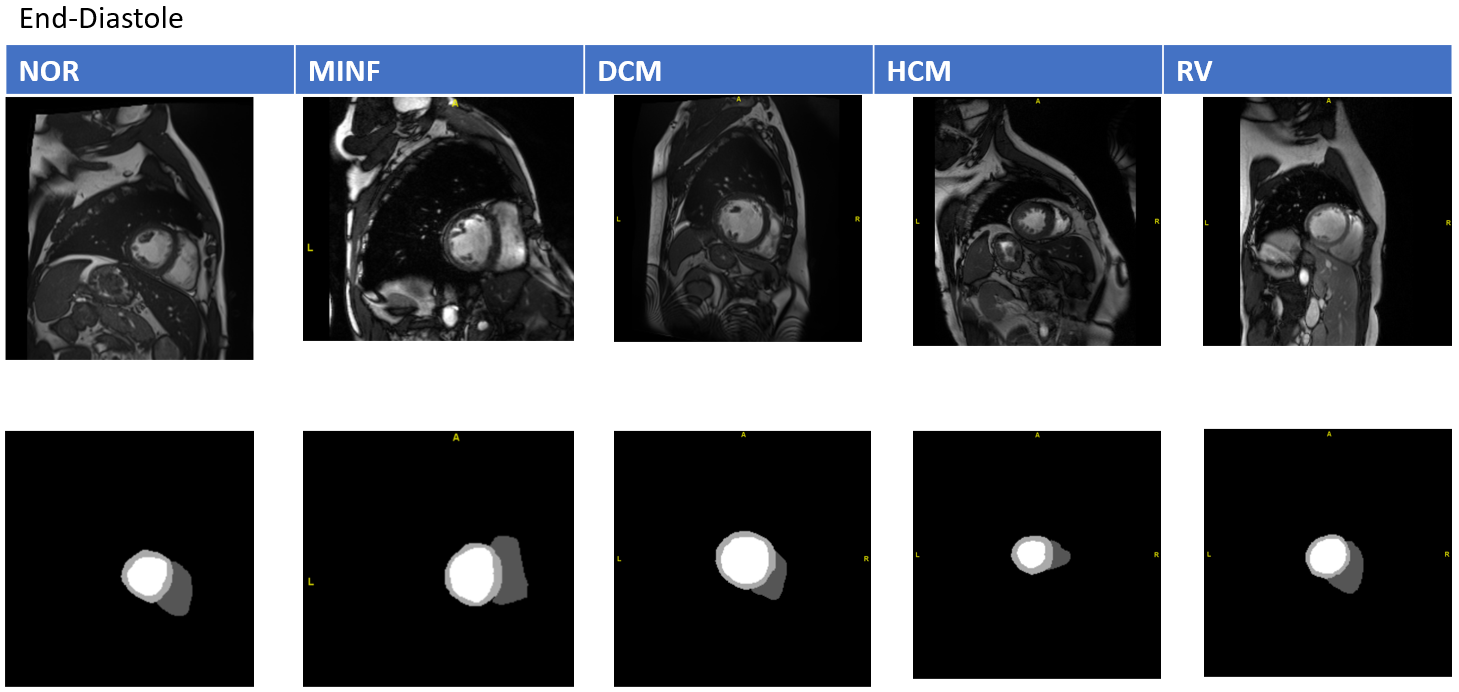
\includegraphics[width=\textwidth]{bab3/ch3-acdc-examples_a.png}
		\centerline{\small (a) End-Diastole (ED) phase}
		\label{fig:ch3-acdc-examples_a}
	\end{minipage}
	
	\vspace{1.5ex}
	
	\begin{minipage}{0.85\textwidth}
		\centering
		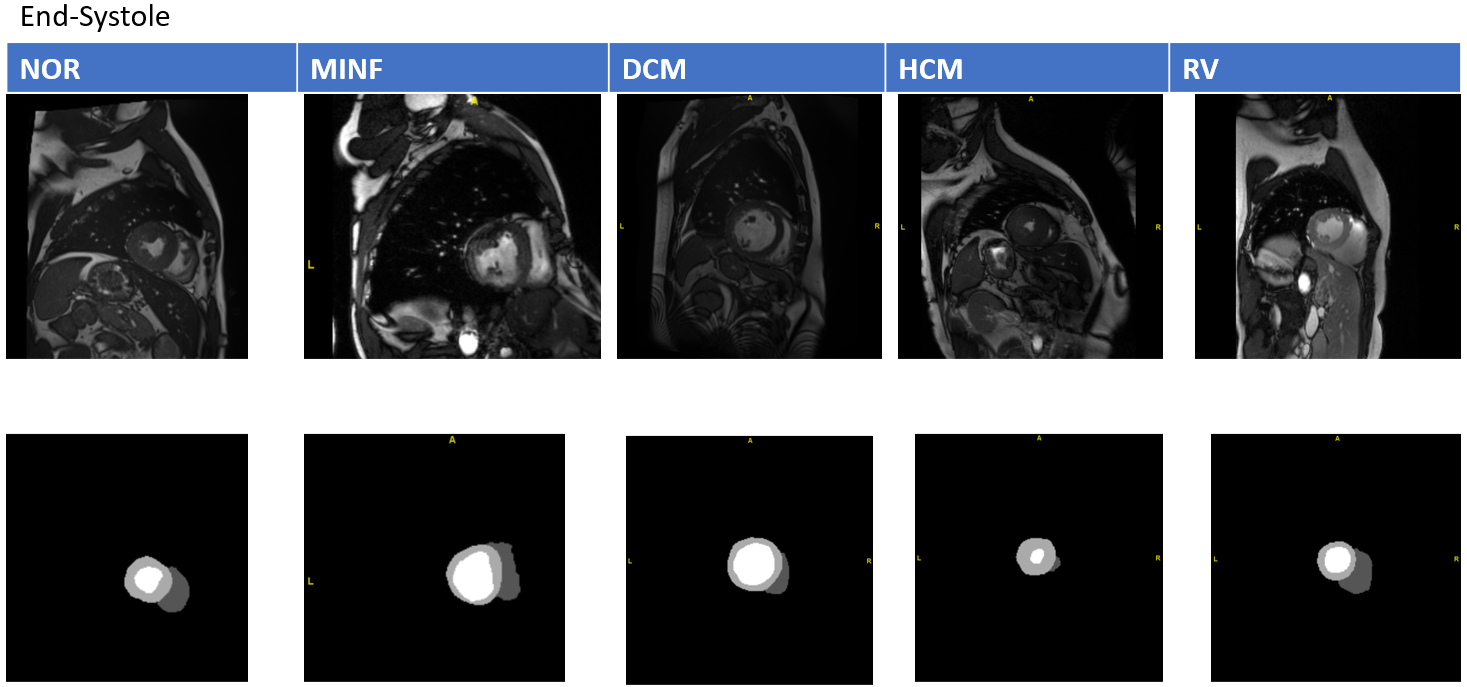
\includegraphics[width=\textwidth]{bab3/ch3-acdc-examples_b.png}
		\centerline{\small (b) End-Systole (ES) phase}
		\label{fig:ch3-acdc-examples_b}
	\end{minipage}
	
	\caption{Representative cine CMR images and corresponding manual annotations from the ACDC dataset \citep{Bernard2018}: (a) End-Diastole (ED) phase, and (b) End-Systole (ES) phase.}
	\label{fig:ch3-acdc-examples}
\end{figure}

\begin{table}[htbp]
\centering
\caption{Characteristics of the ACDC dataset}
\label{tab:acdc-characteristics}
\begin{tabularx}{\textwidth}{p{0.30\textwidth} X}
\toprule
\textbf{Characteristic} & \textbf{Description} \\
\midrule
Dataset & Automated Cardiac Diagnosis Challenge (ACDC) \\
Imaging modality & Cine CMR \\
Number of subjects & 150 \\
Cardiac phases & End-Diastole (ED) and End-Systole (ES) \\
Reference annotations & Left ventricle (LV), right ventricle (RV), and myocardium (MYO) \\
Purpose in this study & Cardiac structure segmentation (Chapters IV and V) \\
\bottomrule
\end{tabularx}

\vspace{4pt}
{\raggedright \footnotesize \textit{Source:} Adapted from \citet{Bernard2018}.\par}
\end{table}

\subsection{Myocardial Pathology Segmentation (MyoPS2020) Dataset}
\label{subsec:myops-dataset}

The Myocardial Pathology Segmentation (MyoPS2020) dataset was used for myocardial scar assessment. Unlike the ACDC dataset, which focuses on cardiac structure segmentation, MyoPS2020 provides complementary multi-sequence CMR images consisting of balanced steady-state free precession (bSSFP), T2-weighted imaging (T2WI), and Late Gadolinium Enhancement (LGE), together with expert annotations of myocardial pathology. These complementary image sequences enable myocardial scar assessment using anatomical and pathological information acquired from different CMR modalities \citep{Zhuang2020}.

Representative examples of the multi-sequence CMR images are presented in Figure~\ref{fig:ch3-myops-examples}, whereas the principal characteristics of the dataset are summarized in Table~\ref{tab:myops-characteristics}.

\begin{figure}[htbp]
	\centering
	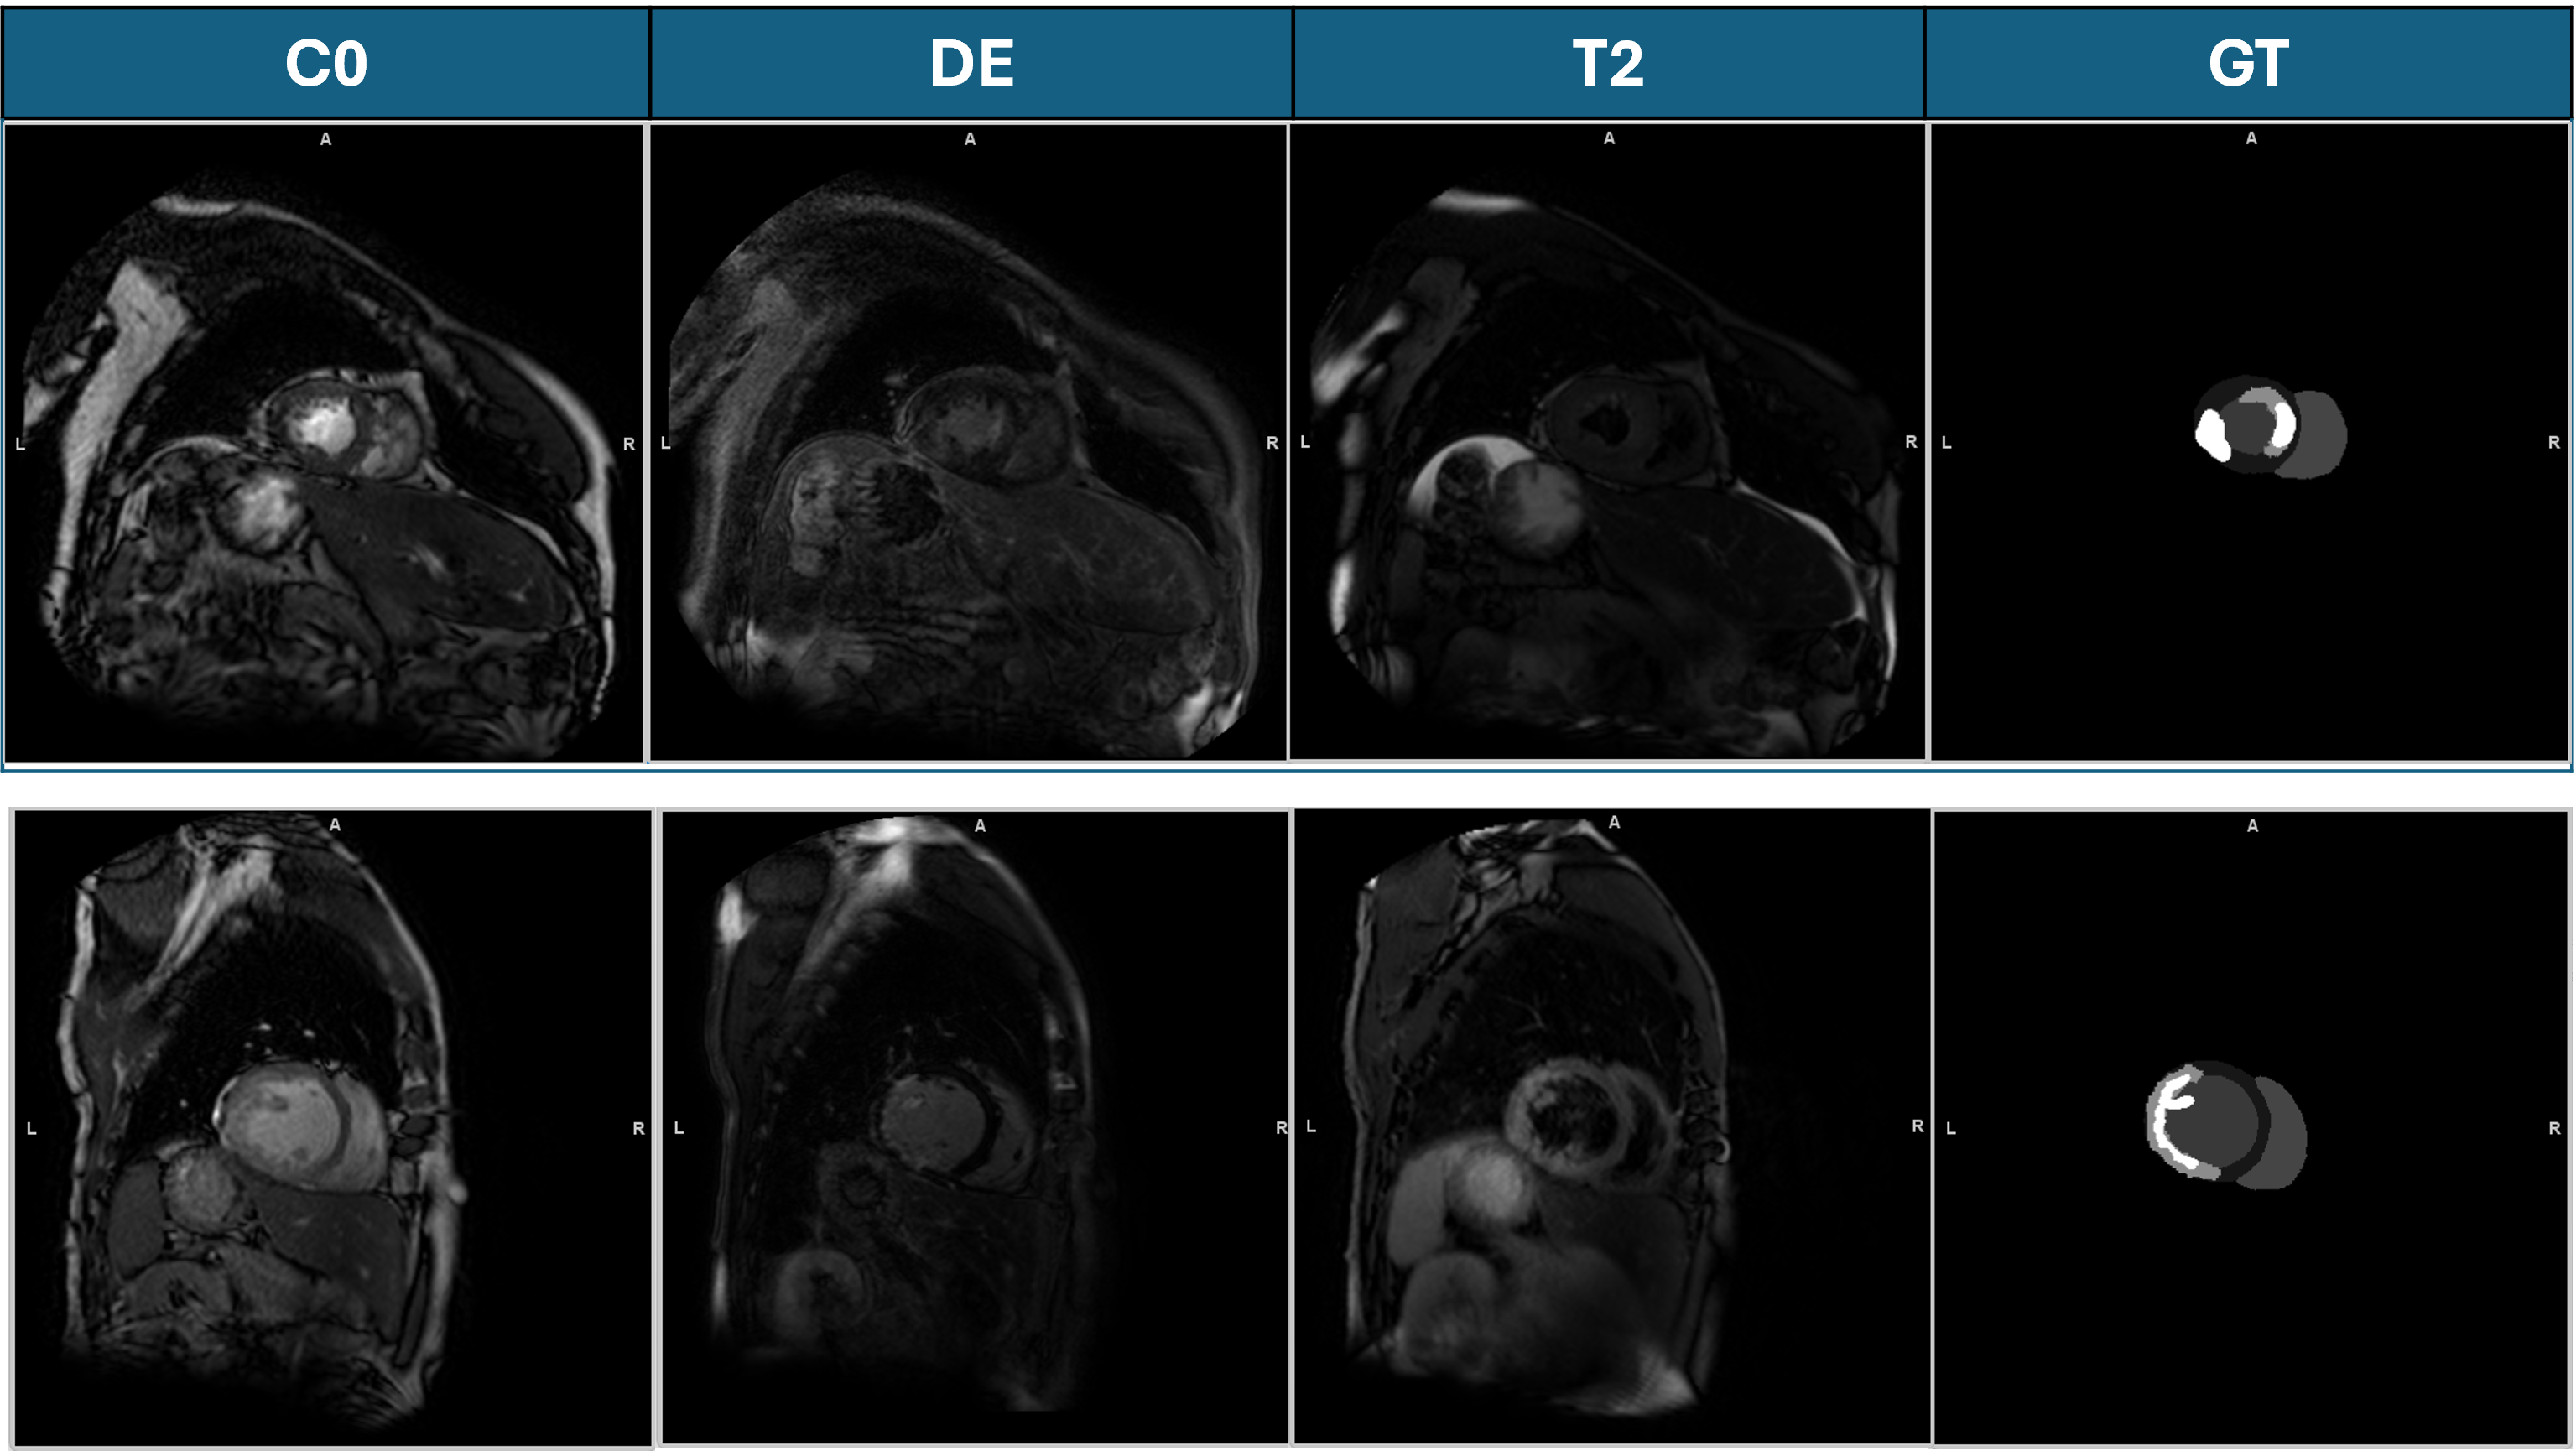
\includegraphics[width=0.86\textwidth]{bab3/ch3-myops-examples.png}
	\caption{Representative multi-sequence CMR images from the MyoPS2020 dataset \citep{Zhuang2020}}
	\label{fig:ch3-myops-examples}
\end{figure}

\begin{table}[htbp]
	\centering
	\caption{Characteristics of the MyOPS2020 dataset}
	\label{tab:myops-characteristics}
	
	% Mengubah tipe kolom X agar rata kiri tanpa membuat spasi melebar
	\begin{tabularx}{\textwidth}{p{0.30\textwidth} >{\raggedright\arraybackslash}X}
		\toprule
		\textbf{Characteristic} & \textbf{Description} \\ \midrule
		Dataset & Myocardial Pathology Segmentation (MyoPS2020) \\
		Imaging modality & Multi-sequence CMR \\
		Number of subjects & 45 \\
		Image sequences & bSSFP, T2WI, and LGE \\
		Reference annotations & Myocardium, edema, and myocardial scar \\
		Purpose in this study & Myocardial scar assessment (Chapter VI) \\ \bottomrule
	\end{tabularx}
\vspace{4pt}
{\raggedright \footnotesize \textit{Source:} Adapted from \citet{Zhuang2020}.\par}
\end{table}

\subsection{Dataset Preparation}
\label{subsec:dataset-preparation}

Before model development, images from the ACDC and MyoPS2020 datasets were prepared using a consistent procedure to ensure compatibility throughout the experiments. Although both datasets underwent image resizing and intensity normalization, the preparation procedure was performed independently according to the objective of each study. The ACDC dataset was prepared for cardiac structure segmentation, whereas the MyoPS2020 dataset was independently prepared for myocardial scar assessment.

Image resizing was first performed to produce a uniform input size for all experiments. Subsequently, intensity normalization was applied to reduce image intensity variations among CMR images acquired from different subjects and imaging conditions. Finally, each dataset was partitioned into training, validation, and testing subsets according to the experimental protocol adopted in this study. The overall dataset preparation procedure is illustrated in Figure~\ref{fig:ch3-dataset-preparation}.

\begin{figure}[htbp]
	\centering
	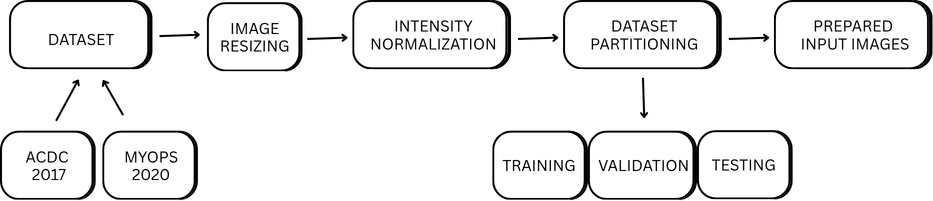
\includegraphics[width=0.86\textwidth]{bab3/ch3-dataset-preparation.png}
	\caption{Overview of the dataset preparation procedure}
	\label{fig:ch3-dataset-preparation}
\end{figure}

As illustrated in Figure~\ref{fig:ch3-dataset-preparation}, both datasets underwent the same general preprocessing stages, including image resizing, intensity normalization, and dataset partitioning. However, each dataset was prepared independently according to its respective research objective, thereby providing standardized inputs for cardiac structure segmentation and myocardial scar assessment.

\section{Cardiac Structure Segmentation}
\label{sec:cardiac-structure-segmentation}

Cardiac structure segmentation represents the first stage of the proposed framework. The objective of this stage is to automatically identify the left ventricle (LV), right ventricle (RV), and myocardium (MYO) from cine CMR images. The resulting myocardium segmentation provides the anatomical information required for the subsequent myocardial scar assessment. Consequently, reliable cardiac structure segmentation establishes the foundation for the overall myocardial infarction assessment framework proposed in this dissertation.

To accomplish this objective, a U-Net-based architecture was adopted as the baseline segmentation framework. Rather than introducing a new network architecture, this study systematically investigates several methodological components that may influence segmentation performance while maintaining the same baseline architecture throughout the experiments. These investigations include activation function selection, fuzzy pooling integration, and loss function investigation. The overall workflow of the cardiac structure segmentation stage is illustrated in Figure~\ref{fig:ch3-cardiac-framework}.

\begin{figure}[htbp]
	\centering
	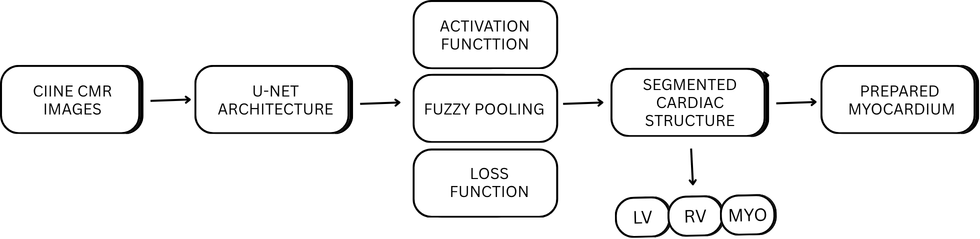
\includegraphics[width=0.86\textwidth]{bab3/ch3-cardiac-framework.png}
	\caption{Overview of the cardiac structure segmentation framework}
	\label{fig:ch3-cardiac-framework}
\end{figure}

\subsection{U-Net Architecture}
\label{subsec:unet-method}

A U-Net architecture was adopted as the baseline segmentation framework for cardiac structure segmentation in this study. Owing to its encoder--decoder architecture with skip connections, U-Net has been widely applied in medical image segmentation for preserving both contextual information and anatomical details \citep{Ronneberger2015}. The theoretical background of the U-Net architecture has been discussed in Chapter~\ref{chap:2} and is therefore not repeated in this chapter.

In this study, the U-Net architecture was applied to segment the left ventricle (LV), right ventricle (RV), and myocardium (MYO) from cine CMR images. To ensure a fair comparison throughout the investigations, the same baseline architecture was consistently maintained in all experiments. Consequently, the methodological investigations presented in this dissertation focus on evaluating different activation functions, pooling strategies, and loss functions without modifying the underlying segmentation network.

The resulting segmentation masks provide the anatomical information required for the subsequent myocardial scar assessment. In particular, the segmented myocardium defines the anatomical region used for myocardial scar analysis, thereby establishing the connection between cardiac structure segmentation and myocardial scar assessment within the proposed framework.

\subsection{Activation Function Selection}
\label{subsec:activation-selection}

The activation function is one of the components that influences how a segmentation network learns from training images. Since different activation functions may produce different learning characteristics, a preliminary investigation was conducted to compare the Rectified Linear Unit (ReLU) and Mish activation functions under the same experimental conditions \citep{Riandini2022IST,Nwankpa2018,Misra2020}.

The objective of this preliminary investigation was to establish the baseline configuration for the proposed cardiac structure segmentation framework. Based on the findings of the preliminary study, the ReLU activation function was selected and subsequently adopted throughout the remaining stages of this dissertation. Consequently, the investigations of fuzzy pooling integration, loss function investigation, and myocardial scar assessment were all performed using the same activation function.

The detailed implementation of the activation function selection is presented in Chapter IV. The selected activation function subsequently serves as the baseline configuration for the methodological investigations presented in Chapters V and VI.

\subsection{Fuzzy Pooling Integration}
\label{subsec:fuzzy-pooling}

Following the establishment of the baseline segmentation framework, the next investigation focused on the pooling strategy used in the U-Net architecture. The pooling strategy influences how image information is preserved when the feature maps are progressively reduced during the learning process. In this study, conventional max pooling and fuzzy pooling were investigated using the same network architecture and experimental configuration \citep{Diamantis2020,Nirthika2022}.

To ensure a fair comparison, only the pooling strategy was changed during this investigation. All principal training settings were maintained consistently throughout the investigation, except for the batch size, which was adjusted to accommodate GPU memory requirements. This experimental design enables the influence of the pooling strategy on cardiac structure segmentation to be evaluated independently.

The detailed implementation of the investigated pooling strategies is presented in Chapter IV. The segmentation framework established through this investigation was subsequently adopted for the loss function investigation described in Section~\ref{subsec:loss-investigation}, thereby maintaining a consistent methodological framework throughout this study.

\subsection{Loss Function Investigation}
\label{subsec:loss-investigation}

Following the investigation of the pooling strategy, the proposed cardiac structure segmentation framework was further developed by investigating different loss functions. The loss function determines how the segmentation network measures the difference between the predicted segmentation and the corresponding reference annotation during training. Since different loss functions emphasize different segmentation characteristics, their selection may influence the final segmentation performance \citep{Ma2021,Azad2023}.

Five representative loss functions were investigated, comprising four established loss functions (Cross-Entropy, Dice, Focal, and Lov\'asz-Softmax) together with the proposed CrossLov Loss. Among these, CrossLov Loss combines Cross-Entropy Loss and Lov\'asz-Softmax Loss into a unified loss formulation to utilize the complementary characteristics of the two loss functions during myocardium segmentation. The proposed CrossLov Loss is mathematically expressed as follows:

\begin{equation}
\mathcal{L}_{\mathrm{CrossLov}}
=
\mathcal{L}_{\mathrm{CE}}
+
\lambda\mathcal{L}_{\mathrm{Lovasz}}
\label{eq:crosslov}
\end{equation}

where $\mathcal{L}_{\mathrm{CE}}$ denotes the Cross-Entropy Loss, $\mathcal{L}_{\mathrm{Lovasz}}$ represents the Lov\'asz-Softmax Loss, and $\lambda$ is the weighting coefficient used to balance the contribution of the two loss components.

To ensure a fair comparison, only the loss function was changed throughout this investigation. The U-Net architecture, activation function, pooling strategy, training dataset, optimizer, learning rate, batch size, and evaluation protocol were maintained unchanged. Consequently, the influence of each investigated loss function could be evaluated independently under the same experimental conditions.

The detailed implementation of the investigated loss functions is presented in Chapter V. The segmentation framework established through this investigation was subsequently incorporated to generate the myocardium segmentation required for myocardial scar assessment, as described in Section~\ref{subsec:scar-preparation}.

\subsection{Preparation for Myocardial Scar Assessment}
\label{subsec:scar-preparation}

The final stage of cardiac structure segmentation prepares the segmented myocardium for myocardial scar assessment. Since myocardial scar develops within the myocardium, accurate segmentation of the myocardium is essential before scar assessment can be performed. Therefore, the myocardium segmentation generated from the previous investigations provides the anatomical information required for the subsequent myocardial scar assessment \citep{Zhuang2020}.

The segmented myocardium is subsequently utilized together with the corresponding multi-sequence CMR images, including balanced steady-state free precession (bSSFP), T2-weighted imaging (T2WI), and Late Gadolinium Enhancement (LGE), to prepare the input for myocardial scar assessment. As illustrated in Figure~\ref{fig:ch3-prepared-myocardium}, this preparation establishes the connection between cardiac structure segmentation and myocardial scar assessment within the proposed framework.

The prepared myocardium is subsequently processed using the myocardial scar assessment framework described in Section~\ref{sec:scar-assessment-method}.

\begin{figure}[htbp]
	\centering
	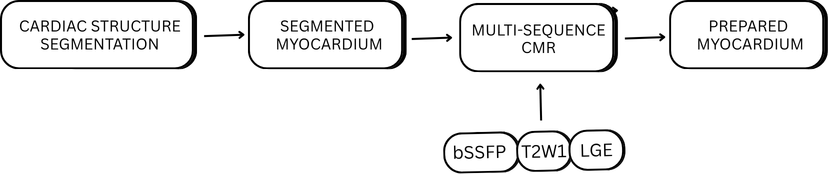
\includegraphics[width=0.86\textwidth]{bab3/ch3-prepared-myocardium.png}
	\caption{Preparation of the myocardium region for myocardial scar assessment}
	\label{fig:ch3-prepared-myocardium}
\end{figure}

\section{Myocardial Scar Assessment}
\label{sec:scar-assessment-method}

Following cardiac structure segmentation, the proposed framework proceeds to myocardial scar assessment using the MyoPS2020 dataset. The objective of this stage is to automatically identify myocardial scar from multi-sequence CMR images and subsequently estimate the corresponding myocardial scar area. Unlike the previous stage, which focuses on cardiac anatomy, this stage focuses on identifying pathological tissue within the segmented myocardium.

The segmented myocardium prepared in Section~\ref{subsec:scar-preparation} provides the anatomical information required for myocardial scar assessment. The corresponding multi-sequence CMR images are subsequently processed using a residual attention-based network to identify myocardial scar. The resulting scar segmentation is then converted into quantitative scar area measurements for myocardial infarction assessment. The overall workflow of this stage is illustrated in Figure~\ref{fig:ch3-scar-framework}.

\begin{figure}[htbp]
	\centering
	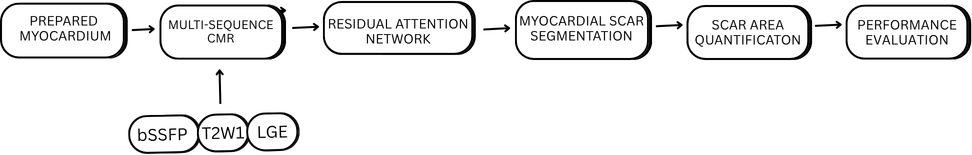
\includegraphics[width=0.86\textwidth]{bab3/ch3-scar-framework.png}
	\caption{Overview of the myocardial scar assessment framework}
	\label{fig:ch3-scar-framework}
\end{figure}

As illustrated in Figure~\ref{fig:ch3-scar-framework}, the prepared myocardium and the corresponding multi-sequence CMR images are processed by the residual attention network to identify myocardial scar. The resulting scar segmentation is subsequently converted into quantitative scar area measurements before being evaluated using the performance metrics described in Section~\ref{sec:performance-evaluation}.

\subsection{Multi-sequence Cardiac Magnetic Resonance Images}
\label{subsec:multi-sequence-method}

Myocardial scar assessment was performed using the MyoPS2020 dataset, which provides three complementary CMR image sequences, namely balanced steady-state free precession (bSSFP), T2-weighted imaging (T2WI), and Late Gadolinium Enhancement (LGE). Each image sequence provides different anatomical and pathological information, allowing the proposed framework to utilize complementary image characteristics during myocardial scar assessment \citep{Zhuang2020}.

Before myocardial scar assessment, the segmented myocardium obtained from the previous stage was associated with the corresponding multi-sequence CMR images. Next, the bSSFP, T2WI, and LGE images were prepared as the input for the proposed scar assessment framework. This preparation enables the network to analyze complementary information from the three CMR image sequences while maintaining their anatomical correspondence.

The overall preparation of the multi-sequence CMR images is illustrated in Figure~\ref{fig:ch3-multi-sequence-preparation}.

\begin{figure}[htbp]
	\centering
	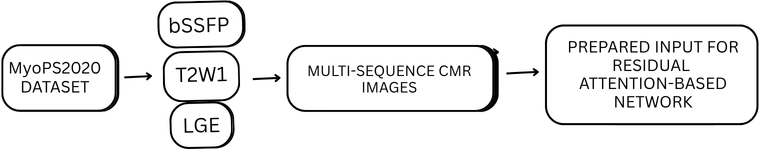
\includegraphics[width=0.86\textwidth]{bab3/ch3-multi-sequence-preparation.png}
	\caption{Preparation of multi-sequence CMR images for myocardial scar assessment}
	\label{fig:ch3-multi-sequence-preparation}
\end{figure}

As illustrated in Figure~\ref{fig:ch3-multi-sequence-preparation}, the three CMR image sequences are combined to provide complementary image information before being processed by the proposed myocardial scar assessment framework. The prepared images are subsequently analysed using the residual attention-based network described in the following section.

\subsection{Residual Attention Network}
\label{subsec:residual-attention-network}

The proposed myocardial scar assessment framework adopts a residual attention-based network to identify myocardial scar from multi-sequence CMR images. Compared with cardiac structure segmentation, myocardial scar exhibits greater variations in shape, size, and image intensity, making automatic segmentation more challenging \citep{He2016,Oktay2018}.

The network adopts an encoder--decoder architecture that integrates residual learning and attention mechanisms. Residual learning facilitates the extraction of image features across multiple network layers, while the attention mechanism guides the network to focus on image regions that are more relevant to myocardial scar. The prepared multi-sequence CMR images described in Section~\ref{subsec:multi-sequence-method} serve as the network input, whereas the corresponding scar annotations are used as the reference during network training.

The residual attention network generates a myocardial scar segmentation that is subsequently used for quantitative scar area estimation, as described in Section~\ref{subsec:scar-area}. The detailed implementation of the proposed network is presented in Chapter VI.

\subsection{Myocardial Scar Segmentation}
\label{subsec:scar-segmentation}

The residual attention network produces a pixel-level segmentation of myocardial scar within the myocardium region prepared in the previous stage. During network training, the predicted scar segmentation is compared with the corresponding reference annotation provided in the MyoPS2020 dataset, enabling the network to learn the spatial distribution of myocardial scar from multi-sequence CMR images \citep{Zhuang2020}.

To ensure that the analysis is focused on the pathological tissue of interest, myocardial scar segmentation is performed within the myocardium identified during the cardiac structure segmentation stage. The segmentation output is represented as a binary scar mask indicating the spatial distribution of myocardial scar within the myocardium.

The resulting scar segmentation serves as the basis for myocardial scar area quantification, which is described in Section~\ref{subsec:scar-area}. The implementation details and experimental evaluation of the proposed scar segmentation framework are presented in Chapter VI.

\subsection{Myocardial Scar Area Quantification}
\label{subsec:scar-area}

Following myocardial scar segmentation, the segmented scar region is converted into a quantitative measurement of myocardial scar area. Quantitative scar area measurement derived from segmentation results has been widely adopted in CMR image analysis to objectively estimate the extent of myocardial scar \citep{Karim2016,Zhuang2020}.

The myocardial scar area is calculated from the binary scar mask generated by the residual attention network. The total number of pixels classified as myocardial scar is first determined and subsequently converted into a physical area using the spatial resolution of the corresponding CMR image. The myocardial scar area is calculated as

\begin{equation}
A_{\mathrm{scar}} = N_{\mathrm{scar}} \times A_{\mathrm{pixel}}
\label{eq:scar-area}
\end{equation}

where $A_{\mathrm{scar}}$ denotes the estimated myocardial scar area (mm$^2$), $N_{\mathrm{scar}}$ is the total number of pixels classified as myocardial scar, and $A_{\mathrm{pixel}}$ represents the physical area corresponding to a single image pixel (mm$^2$/pixel).

The estimated myocardial scar area obtained from the proposed framework was subsequently compared with the corresponding reference measurements using MAE, RMSE, PCC, and Bland--Altman analysis, as described in Section~\ref{sec:performance-evaluation}.

\section{Experimental Design}
\label{sec:experimental-design}

The experimental design adopted in this dissertation was developed to systematically evaluate the contribution of each methodological component within the proposed deep learning framework for CMR image analysis. Rather than modifying several components simultaneously, each investigation focused on a single methodological component while maintaining the remaining experimental settings unchanged. This experimental strategy enables the influence of each investigated component to be evaluated independently and ensures that the observed performance differences are attributable to the investigated method.

As illustrated in Figure~\ref{fig:ch3-experimental-design}, the study was conducted through four sequential stages. A preliminary investigation was first performed to establish the baseline segmentation framework through activation function selection. Following this, the proposed framework was progressively developed through fuzzy pooling integration and loss function investigation before being applied to myocardial scar assessment and quantitative scar area estimation. The corresponding methodological components investigated at each stage are summarized in Table~\ref{tab:experimental-design}.

\begin{figure}[htbp]
\centering
\fbox{\parbox{0.86\textwidth}{\centering Insert final experimental design adopted in this study. here}}
\caption{Experimental design adopted in this study.}
\label{fig:ch3-experimental-design}
\end{figure}
%\noindent\textit{Source: Developed by the author.}

\begin{table}[htbp]
\centering
\caption{Overview of the experimental design adopted in this study}
\label{tab:experimental-design}
\begin{tabularx}{\textwidth}{
		>{\raggedright\arraybackslash}p{0.18\textwidth}
		>{\raggedright\arraybackslash}p{0.30\textwidth}
		>{\raggedright\arraybackslash}X
	}
	\toprule
	\textbf{Stage} & \textbf{Methodological Component} & \textbf{Purpose} \\
	\midrule
	Preliminary Study & Activation function selection & Establish the baseline segmentation framework \\
	Stage I & Fuzzy pooling integration & Investigate the influence of the pooling strategy on cardiac structure segmentation \\
	Stage II & Loss function investigation & Evaluate different loss functions for cardiac structure segmentation \\
	Stage III & Myocardial scar assessment & Perform myocardial scar segmentation and quantitative scar area estimation \\
	\bottomrule
\end{tabularx}
\end{table}
%\noindent\textit{Source: Developed by the author.}

As summarized in Figure~\ref{fig:ch3-experimental-design} and Table~\ref{tab:experimental-design}, the proposed framework was developed progressively, where the outcome of each stage served as the basis for the subsequent investigation. This experimental design ensures methodological consistency throughout the dissertation while enabling each investigated component to be evaluated independently.

\section{Performance Evaluation}
\label{sec:performance-evaluation}

The proposed framework was evaluated using quantitative performance metrics selected according to the objective of each stage of the study. Since this dissertation consists of cardiac structure segmentation, myocardial scar segmentation, and myocardial scar area quantification, different evaluation metrics were adopted to assess segmentation accuracy, boundary agreement, structural similarity, and quantitative measurement agreement. The mathematical formulations of these metrics have been presented in Chapter~\ref{chap:2}, whereas their application in this study is summarized in Table~\ref{tab:evaluation-metrics}.

\begin{sidewaystable}[htbp]
	\centering
	\small
	\caption{Performance evaluation metrics adopted in this study}
	\label{tab:evaluation-metrics}
	
	\renewcommand{\arraystretch}{1.3}
	\begin{tabularx}{\linewidth}{>{\raggedright\arraybackslash}p{0.20\linewidth} >{\raggedright\arraybackslash}p{0.20\linewidth} p{0.12\linewidth} >{\raggedright\arraybackslash}X}
		\toprule
		\textbf{Task} & \textbf{Output} & \textbf{Metric} & \textbf{Purpose} \\ \midrule
		
		Cardiac structure segmentation & 
		LV, RV, and myocardium & 
		IoU \newline HD & 
		Measure regional agreement \newline Assess boundary accuracy \\ \addlinespace % <-- Diganti ke \addlinespace
		
		Myocardial scar segmentation & 
		Myocardial scar segmentation & 
		DSC \newline IoU \newline HD \newline SSIM & 
		Evaluate segmentation overlap \newline Measure regional agreement \newline Assess boundary accuracy \newline Evaluate structural similarity \\ \addlinespace % <-- Diganti ke \addlinespace
		
		Myocardial scar area quantification & 
		Myocardial scar area (mm$^2$) & 
		MAE \newline RMSE \newline PCC \newline Bland--Altman & 
		Measure absolute estimation error \newline Measure the magnitude of estimation error while penalizing larger errors \newline Evaluate measurement correlation \newline Assess agreement between estimated and reference scar area \\ \bottomrule
	\end{tabularx}
\end{sidewaystable}

As summarized in Table~\ref{tab:evaluation-metrics}, segmentation performance was evaluated using overlap-based, boundary-based, and structural similarity metrics, whereas myocardial scar area quantification was evaluated using quantitative agreement analysis. The detailed experimental results obtained using these evaluation metrics are presented in Chapters IV, V, and VI.